\chapter{Bringing Storm to Multi-core}

The following chapter explains the design of Storm-MC. We describe how Apache Storm behaves on multi-core machines (\ref{sec:storm_on_mc}), how the Storm architecture was ported over to multi-core (\ref{sec:storm_mc_arch}), and we list feature differences between Apache Storm and Storm-MC (\ref{sec:differences}).

\section{Apache Storm on Multi-core}
\label{sec:storm_on_mc}

To begin, we discuss why Apache Storm does not perform optimally on a single multi-core machine. Storm can be ran in local mode where it emulates execution on a cluster. This mode exists so that it is possible to debug and develop topologies without needing access to a cluster. However, there are several reasons why the local mode is not as performant as it could be.

\subsection{Tuple Processing Overhead}

\begin{figure}[!htb]
	\centering
	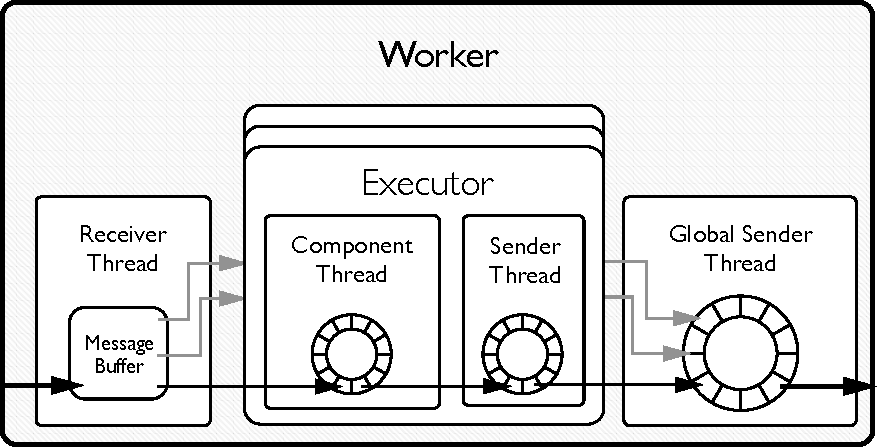
\includegraphics[scale=0.7]{pdf/worker_inside.pdf}
	\caption{Tuple processing in Apache Storm.}
	\label{fig:worker_inside}
\end{figure}

Figure \ref{fig:worker_inside} shows how tuple processing is implemented inside a Storm worker process. The tuple is read from a message buffer by the receiver thread of the worker and put on a receive queue of the target executor. The tuple is then picked up by the component thread of the executor for task execution.

After the component thread has executed the task it puts the tuple on the executor send queue. There, it is picked up by the executor sender thread which puts the tuple on the global send queue of the worker. Finally, the global sender thread of the worker serialises the tuple and sends it downstream.

Alternatively, if the tuple is forwarded to an executor in the same worker process it is put on the receive queue of the corresponding executor directly after task execution.

The queues used in Storm are implemented as ring buffers using the LMAX Disruptor library \citep{LMAXDisruptor}. Detailed background on how Disruptor works and its performance benchmarks can be found in \citep{Thompson_Farley_Barker_Gee_Stewart_2011}.

There is significant overhead required to simulate sending tuples to executors in other worker nodes. For one, there is the overhead from the tuple passing through the three queues of a worker. The authors of LMAX Disruptor showed that a three step pipeline has half the throughput of a single consumer-producer pipeline \citep{DisruptorWiki}.

Furthermore, to emulate over-the-network messages Storm uses a \texttt{Hashmap} of \texttt{LinkedBlockingQueue}s which according to \cite{Thompson_Farley_Barker_Gee_Stewart_2011} has several orders of magnitude lower performance than the Disruptor. Due to less write contention, lower concurrency overhead, and being more cache-friendly the Disruptor pattern can offer latency of inter-thread messages lower than 50 nanoseconds and a throughput of over 25 million messages per second.

\subsection{Thread Overhead}

\begin{description}
	\item[Acker Bolt] \hfill \\
	The Acker is included in every topology. The Acker bolt can be disabled via the configuration file. In such a case it is mostly idle since it does not receive any messages but it can still use up resources especially if it waits for messages using a busy waiting strategy.
	\item[Heartbeats \& Timers] \hfill \\
	Every worker has a heartbeat thread that simulates sending heartbeat messages to the Nimbus node. It does this by writing to a local cache which is persisted to a file by a write on every heartbeat. Since the write is implemented using the \texttt{java.io} package the write is blocking - the thread cannot continue until the write is completed. While heartbeats are essential in cluster mode to signal the node being alive, there is no need for them in local mode.
	\item[Zookeeper Emulation] \hfill \\
	More overhead is produced by a local Zookeper server which emulates the Zookeeper nodes of a cluster. Running the Zookeeper server is a massive addition to the list of overheads as shown in the following paragraphs. The purpose of Zookeeper is to maintain states of running topologies and nodes of the cluster. As we will show in the following sections maintaining this state on multi-core is not necessary.
\end{description}

During profiling we found that a topology with one worker and three executors was being executed with 55 threads (not including system JVM threads and threads created by the profiler). Table \ref{table:breakdown} shows a breakdown of what the individual threads were used for.

\begin{table}[htb!]
\centering
\small
\begin{tabular}{@{}ll@{}}
    \textbf{Spout Parallelism} & \textbf{\# of Threads} \\ \toprule
    Main Thread & 1  \\
	Worker Sender \& Receiver Threads & 2  \\
    Acker \& System Component Threads & 2  \\
    Executor Component Threads & 3  \\
    Executor Sender Threads & 5  \\
    Various Timers \& Event Loops & 14  \\
    Zookeper Server & 28  \\
\end{tabular}
\caption{Breakdown of threads used by Storm to execute a 3-component topology.}
\label{table:breakdown}
\end{table}

To find out what state the threads were actually in at any given time the topology was executed for three minutes and a JVM thread dump was recorded every second. The average results of this experiment can be observed in table \ref{table:dump} and the state distribution over time can be seen in Figure \ref{fig:dump-plot}.

\begin{table}[htb!]
\centering
\small
\begin{tabular}{@{}lc@{}}
    \textbf{Spout Parallelism} & \textbf{\# of Threads} \\ \toprule
    RUNNABLE & 8  \\
	TIMED WAITING & 22  \\
    WAITING & 25  \\
\end{tabular}
\caption{Average number of recorded thread states over a three minute period.}
\label{table:dump}
\end{table}

<<dump-plot, echo=FALSE, cache=TRUE, fig.cap="Thread state distribution over time.", fig.pos="!htb", fig.height=3>>=
@

Even though three minutes may seem to be a very short amount of time the fact that there is almost no variation shows that it is sufficient. As can be seen from the table, most of the threads were either in state \texttt{WAITING} or \texttt{TIMED WAITING}. According to the Java documentation on thread states \citep{JavaThreads} these two states are used for threads that are waiting for an action from a different thread and cannot be scheduled by the scheduler until that action is executed.

On average there were eight threads in state \texttt{RUNNABLE} which JVM uses to mark threads which are executing on the JVM and are possibly waiting for resources from the operating system (OS) such as processor \citep{JavaThreads}. Hence, these are threads directly competing to be scheduled by the OS. This means that for three components running in parallel there are five threads doing potentially unnecessary work.

In the subsequent sections we will show that these threads were in fact unnecessary and we will discuss how the number of threads was reduced. In fact, to execute the same topology on Storm-MC requires only 5 threads.

\section{Storm-MC Design}
\label{sec:storm_mc_arch}

The design we adopted for porting worker nodes is to only have one worker executing all the executors of a topology. This design simplified the communication model and removed unnecessary abstractions.

Additionally, the code for the Nimbus service was merged with the worker. This was done because there is no need to run Nimbus and worker specific code in parallel. Once Nimbus sets up the topology, all the work is done by the worker. Hence they can be executed serially.

\subsection{Nimbus}

Unlike Storm executing on a cluster, Storm-MC does not support running multiple topologies at the same time. However, to do that one only needs to run the topology in a separate process. This is because unlike when executing on the cluster different topologies do not need to share any state and it is more natural to execute them as separate processes.

This has the added benefit of each process having its own part of main memory thus reducing cache conflicts as shown in \citep{Chandra:2005:PIC:1042442.1043432} and providing higher security by not having different topologies share memory space. Additionally, if a single thread of one topology is blocking it does not block other topologies.

Storm-MC does not support topology scheduling. Since within one process there is always only one topology running at a time and the hardware configuration of the machine does not change, the parallelism is clearly defined by the number of executors per component specified in the topology configuration.

One way to implement scheduling could be to pin threads to specific cores. Unfortunately, Java does not provide support for CPU affinity, the assignments are handled automatically by the JVM. Potentially, this could be achieved by using C or C++, both of which support CPU affinity, but this was not implemented in Storm-MC.

The role of Nimbus in Storm-MC has effectively been reduced to validating the topology and passing it along to the worker source code which handles topology execution.

\subsection{Worker}

In Apache Storm, a worker node runs the supervisor daemon, which in turns launches worker processes which run executors which execute tasks. In Storm-MC, however, there is only one worker process which runs all the executors and their tasks. This design has several benefits:

\begin{itemize}
	\item All the inter-thread communication occurs within one worker process.
	\item The supervisor daemon can be removed as there is no need to synchronise or monitor workers.
	\item There is no need to simulate over-the-network message passing.
	\item Message passing between executor threads within a worker stays the same as in Apache Storm.
\end{itemize}

A comparison of an Apache Storm worker node and its Storm-MC equivalent is shown in Figure \ref{fig:comparison}.

\begin{figure}[!htb]
\centering
\begin{subfigure}{.5\textwidth}
  \centering
  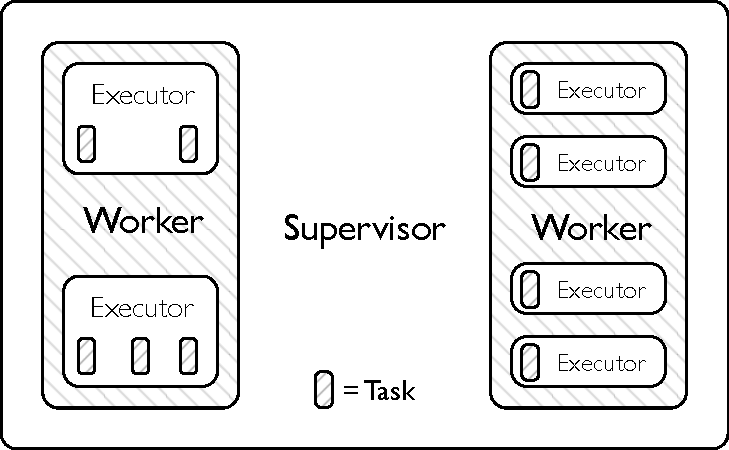
\includegraphics[width=0.95\linewidth]{pdf/distributed_worker.pdf}
  \caption{Worker node in Apache Storm.}
  \label{fig:comparison1}
\end{subfigure}%
\begin{subfigure}{.5\textwidth}
  \centering
  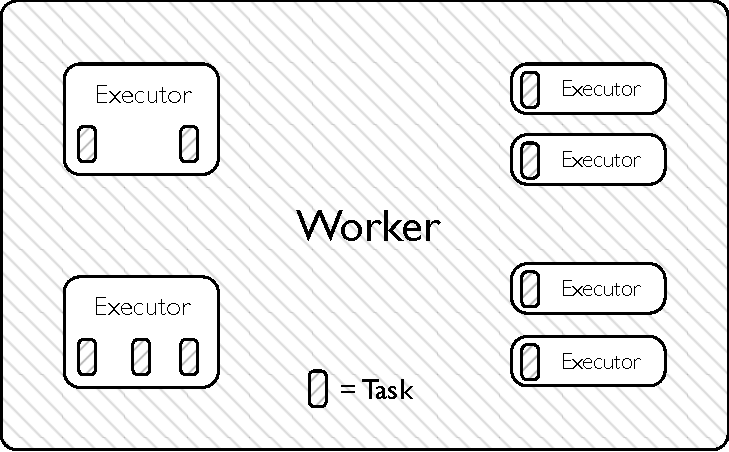
\includegraphics[width=0.95\linewidth]{pdf/local_worker.pdf}
  \caption{Worker node equivalent in Storm-MC.}
  \label{fig:comparison2}
\end{subfigure}
\caption{Comparison of a worker in Storm and Storm-MC}
\label{fig:comparison}
\end{figure}

The role of the worker is to launch executors and provide them with a shared context through which they can communicate. This is done with a map of executor identifiers to Disruptor queues which the executors use to pass tuples between each other.

\todo{Write about disruptor here.}

Moreover, the worker contains a map of components to streams and fields. This map is used by components to figure out which components subscribe to streams they produce.

Additionally, a worker has a user timer which components can use to get tick tuples at regular intervals.

Finally, a worker contains shared resources which can be used by the executors. One such resource is a configurable-size thread-pool \texttt{ExecutorService}. Executors can use these via the topology context to execute some computation on a separate thread.

\todo{Refactor below section}

\subsection{State}

As mentioned before, Storm-MC is completely stateless. The cluster state that was managed by Zookeeper in Apache Storm was completely stripped away. This state was only relevant when multiple topologies were sharing resources.

\subsection{Serialisation}

Great amount of work was put into removing the dependency of Storm-MC on Apache Thrift. This was mostly done to reduce code bloat and remove an unnecessary dependency since there is no serialisation required in a multi-core environment.

This required refactoring all the data types generated automatically by Thrift. This also significantly reduced the size of the codebase and made the code more readable and self-documenting than the code generated by Thrift.

\section{Implementation Details}

\begin{figure}[!htb]
	\centering
	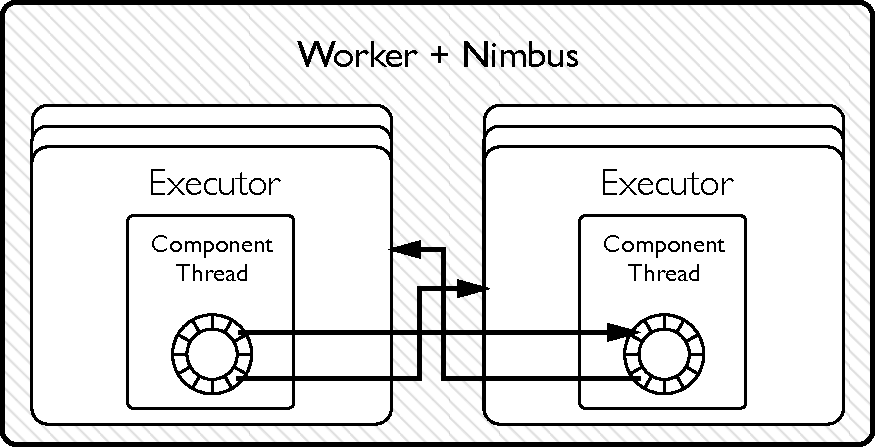
\includegraphics[scale=0.7]{pdf/worker_inside_mc.pdf}
	\caption{Tuple processing in Storm-MC.}
	\label{fig:worker_inside_mc}
\end{figure}

The implementation of tuple processing in Storm-MC is depicted in Figure \ref{fig:worker_inside_mc}. As can be seen from the figure, the queues used for remote message sending were stripped away and there is only one Disruptor queue for every executor. Once an executor is done processing a tuple it simply puts it on the Disruptor queue of its downstream bolts.

Thus the tuple processing in Storm-MC is a variant of multiple producer single consumer problem. We considered several other options such as \texttt{ArrayBlockingQueue} when implementing the tuple processing mechanism. However, the Disruptor shows superior throughput and latency compared to alternative solutions \citep{DisruptorWiki}.

\todo{Storm-MC requires one thread per component, user timer and main thread}

\subsection{Nimbus}

\subsection{Worker}

As mentioned in previous chapter Storm-MC was implemented with only one worker per topology. This worker then exposes a common context to all the executors.

\subsection{Executor Receive Queues}

Worker stores a map of executor ids to receive queues. These are then used by executors to pass tuples between each other. As discussed in the previous chapter, the queues are implemented as Disruptor ring buffers. The way this works is as follows:

The target executor waits at for the next entry of the ring buffer to become available. There are four different waiting strategies an executor can employ:

\begin{description}
	\item[BlockingWaitStrategy] \hfill \\
	This strategy uses a lock and a condition variable. 
	\item[YieldingWaitStrategy] \hfill \\
	This strategy initially spins for hundred iterations and then uses \texttt{Thread.yield()}.
	\item[SleepingWaitStrategy] \hfill \\
	This strategy initially spins for hundred iterations, then uses \texttt{Thread.yield()}, and finally uses \texttt{LockSupport.parkNanos(1L)} to sleep.
	\item[BusySpinWaitStrategy] \hfill \\
	In this strategy the thread is in a so-called tight loop, where it checks whether a new entry is available, breaks out if it is. Otherwise it continues looping.
\end{description}

\subsection{Executor}

An executor is implemented as a single thread of execution. This thread consumes a batch of tuples from the Disruptor queue when it becomes available, performs the tasks of a component it represents, and finally places the newly produced tuples on the Disruptor queue of other executors.

In Apache Storm, an executor runs two threads in parallel. One that picks up new tuples from the receive queue

\todo{Describe how executor is implemented - Thread vs Executor}

\section{Differences between Apache Storm and Storm-MC}
\label{sec:differences}

The codebase of Apache Storm is fairly large - 54,985 lines of code as reported by \texttt{cloc} \citep{Cloc}. Thus we had to prioritise features that were ported over to Storm-MC. Table \ref{table:features} presents a list of Storm features and shows which were ported over to Storm-MC and which were not.

\begin{table}[h!]
\centering
\small
\begin{tabular}{@{}lcc@{}}
    \textbf{Feature} & \textbf{Apache Storm} & \textbf{Storm-MC} \\ \toprule
    Multi-language Topologies & \cmark & \cmark \\
    Hooks & \cmark & \cmark \\
    Metrics & \cmark & \cmark \\
    Tick Tuples & \cmark & \cmark \\
    Multiple Topologies & \cmark & \xmark \\
	Trident API & \cmark & \xmark \\
    System Bolt & \cmark & \xmark \\
    Built-in Metrics & \cmark & \xmark \\
    Nimbus as a Server & \cmark & \xmark \\
\end{tabular}
\caption{Feature comparison of Apache Storm and Storm-MC.}
\label{table:features}
\end{table}
